\begin{multicols}{2}
\textbf{Ingredients}
\begin{itemize}
\item 1 onion 
\item 2 lbs stew beef 
\item 1 can diced tomatoes
\item 2 medium zucchini 
\item 3 russet potatoes (medium/medium large) 
\item 1 lb baby carrots 
\item 2 cans tomato sauce (8 oz each) 
\item 1 can of corn (with water) 
\item $\sim 5$ cloves of garlic (minced)
\item 4-5 cups of water (enough to fill $\frac{1}{4}$ inch from rim of crock pot.)

\item 6-7 cubes of beef bullion 
\item 2 tsp. salt (more to taste) 
\item 1 tsp. black pepper
\item 1 tsp. thyme
\item 3 bay leaves 


\end{itemize}


\columnbreak
\textbf{Procedure:}
\medskip


\begin{enumerate}
\item \textbf{\textit{Note:}} This is a MASSIVE recipe. This will fill an 8-quart slow cooker to the brim. 
\item Dice onion, cube potatoes and beef, chop carrots in half, cut zucchini into bite-sized pieces. Add to crock pot. Add canned items, bullion, and spices then fill with water and give it a good stir. 


\medskip
\item Cook on low in crock pot for approximately 8 hours for best results. I usually start it in the morning to have it ready for dinner. 
  
\end{enumerate}

\end{multicols}




%\begin{center}
%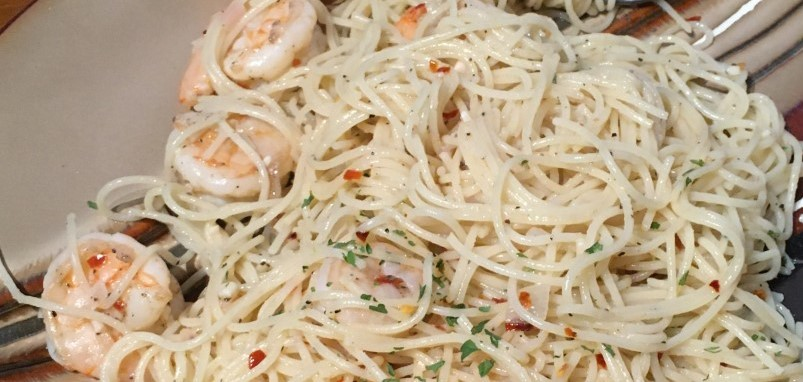
\includegraphics[scale=0.65]{Pasta/Shrimp Scampi/Shrimp Scampi.jpg}
%\end{center}
